\section{Datenbankmodelle}
\label{datenmodelle}
In diesem Abschnitt werden die Grundlagen des relationalen und Graph-basierten Datenbankmodell skizziert. Diese sind im Rahmen dieser Arbeit von wesentlicher Bedeutung. Schließlich vereint die in \compref{chap:db2graph} beschriebene Graph-Erweiterung sowohl Elemente des relationalen, als auch des Graphmodells.

Um einen Überblick über diese Modelle zu geben, werden beide unter einem jeweiligen Aspekt des Modells einander gegenüber gestellt. Zu den Aspekten dieses Vergleichs gehören: 

\begin{itemize}
    \item Herkunft \& Verbreitung,
    \item Struktur \& Schema,
    \item Beziehungen und
    \item Abfragesprachen.
\end{itemize}

Die Beschränkung auf diese Aspekte wurde dabei vorgenommen, da ein tiefgreifender Vergleich beider Modelle über den Rahmen der Arbeit hinausgehen würde. Dieser Abschnitt vermittelt hierbei die für das Verständnis der Arbeit benötigten Informationen bezüglich der Datenbankmodelle. Abschließend werden die wichtigsten Ergebnisse nochmals kurz zusammengefasst.  

\subsection{Herkunft \& Verbreitung}
In diesem Unterabschnitt wird auf die Herkunft und aktuelle Verbreitung der beiden Modell eingegangen. Die Verbreitung wird dabei an der aktuellen Verbreitung von relationalen und Graph-Datenbanksystemen gemessen. 

\subsubsection{Relationales Modell}
Das relationale Modell hat seinen Ursprung in den 1970er Jahren \cite{rdbms_history}. Seine Grundlagen wurden dabei erstmals in \cite{codd_relational_model} von \citeauthor{codd_relational_model} umrissen. In den folgenden Jahren  wurde beim IBM Research unter dem Namen \textit{System R} ein erstes relationales Datenbanksystem entwickelt \cite{rdbms_history}. Hervorzuheben ist hierbei, dass die Paper die im Zuge der Forschung und Entwicklung am \textit{System R} veröffentlicht wurden, der Öffentlichkeit frei zur Verfügung gestellt wurden \cite{rdbms_history}. Wodurch auch andere Unternehmen auf diesem Wissen aufbauen konnten.

Heute haben relationale Datenbanksysteme eine große Verbreitung gefunden, siehe \autoref{fig:dbms_marketshare}. So sollen nach \cite{db_engines_ranking_july} relationale Datenbanksysteme 72,7 \% des gesamten Datenbankmarktes ausmachen (Stand Juli 2021). Folglich kann dem relationalen Modell und relationalen Datenbanksystemen die marktbeherrschende Rolle zugeschrieben werden.

\begin{figure}[ht]
    \centering
    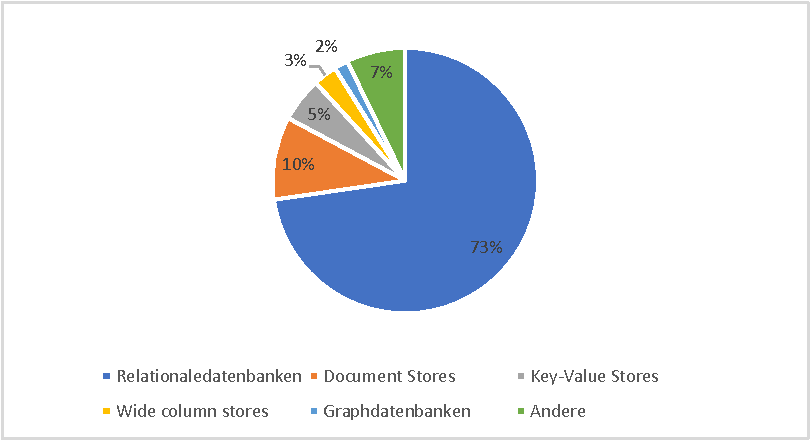
\includegraphics[width=\textwidth]{images/marketshare_dbms.pdf}
    \caption{Marktanteile nach Datenbankmanagementsystem-Kategorie}
    \label{fig:dbms_marketshare}
    \vspace{1em}
    \textit{Bei den hier abgebildeten Werten handelt es sich um die aufgerundeten Werte aus} \cite{db_engines_ranking_july}\textit{.}
\end{figure}

\subsubsection{Graphmodell}
Das Graphmodell als Datenbankmodell hat seinen Ursprung in der heutigen Form im Jahr 1999 \cite{gdbms}. Dabei wurde das Graphmodell mit der Motivation entwickelt, vermeintliche Nachteile oder Probleme des relational Modells auszuräumen \cite{gdbms}.

Graphdatenbanksysteme und das Graphmodell sind heute als vergleichbar junge Technologien noch nicht so weit verbreitet wie beispielsweise, dass relationale Modell. Mit 1,7 \% Marktanteil ordnen sich Graph-Datenbanksysteme noch weit hinter anderen Technologien ein, wie \textit{Document Stores}, \textit{Key-Values Stores} oder \textit{Wide column stores} \cite{db_engines_ranking_july}, siehe \autoref{fig:dbms_marketshare}. Jedoch haben Graphdatenbanksysteme seit 2013 einen erheblichen Aufschwung in ihrer Popularität erfahren \cite{db_engines_ranking_july}. 

\subsection{Struktur \& Schema}
\label{datenmodelle:structure}
Im Rahmen dieses Abschnitts wird auf die vorhandenen Strukturen der Datenbankmodelle eingegangen. Darüber hinaus wird auch das zugrundeliegende Schema genauer erläutert. 

\subsubsection{Relationales Modell}
\label{datenmodelle:structure:relational}
Im Zentrum des relationalen Modells steht das sogenannte Informationsprinzip \cite{rdbms_history}. Dies beschreibt, dass alle Informationen in einer Datenbank ausschließlich in exakt einer Weise repräsentiert werden dürfen \cite{codd_relational_model}. Informationen werden dabei in Form von Tupeln und Relationen organisiert \cite{codd_relational_model}. Für deren Organisation stellen relationale Datenbanksysteme Tabellen, Spalten und Zeilen als Strukturen bereit \cite{rdbms_history}. So werden auf Basis des Informationsprinzips, alle Informationen als Werte in einer Zelle einer bestimmten Tabelle repräsentiert \cite{rdbms_history}. Dadurch lassen sich beispielsweise alle Entitäten vom Entitätstyp Auto in einer relationalen Tabelle abbilden, siehe \autoref{tab:auto_tabelle}. 

\begin{table}[ht]
    \centering
    \begin{tabular}{c|c|c|c}
    \hline
    \rowcolor[HTML]{EFEFEF} 
    \multicolumn{1}{l|}{\cellcolor[HTML]{EFEFEF}\textbf{Fahrzeugnummer}} & \multicolumn{1}{l|}{\cellcolor[HTML]{EFEFEF}\textbf{Marke}} & \multicolumn{1}{l|}{\cellcolor[HTML]{EFEFEF}\textbf{Model}} & \multicolumn{1}{l}{\cellcolor[HTML]{EFEFEF}\textbf{Baujahr}} \\ \hline
    FZ-123456789 & Toyota & Starlet & 1997 \\
    FZ-234567890 & Nissan & Leaf & 2018 \\
    FZ-345678912 & VW & ID3 & 2020 \\
    FZ-456789123 & Ford & Fiesta & 2001 \\
    ... & ... & ... & ... \\ \hline
    \end{tabular}
    \caption{Beispiel relationale Tabelle}
    \vspace{0.1em}
    \textit{Hier wird eine einzelne relationale Tabelle gezeigt. Die gezeigten Daten repräsentieren dabei verschiedene Entitäten des Typs Auto.}
    \label{tab:auto_tabelle}
\end{table}

Das relationale Modell setzt bei der Datenhaltung allerdings ein striktes Schema voraus \cite{rdbms_book}, weil Informationen nach dem Informationsprinzip ausschließlich auf eine Weise repräsentiert werden dürfen \cite{rdbms_history}. Es verlangt somit eine homogene Darstellung der Daten. Allerdings sind viele Daten in der realen Welt heterogen. Dies hat zu Folge, dass Daten einen sogenannten Normalisierungsprozess durchlaufen müssen \cite{rdbms_book}. Bei diesem Prozess werden die Daten in die sogenannte dritte Normalform (3NF) gebracht, wodurch jegliche Anomalien vermieden werden können \cite{rdbms_book}. So können letztendlich die Informationen einer Entität in einem homogenen Typschema abgebildet werden. 

\subsubsection{Graphmodell}
Die Grundlage des Graphmodells stellen sogenannte Vertexes und Edges dar, auf Deutsch Knoten und Kanten \cite{gdbms}. Diese Vertexes und Edges bilden dabei zusammen einen sogenannten Graphen. So werden in einem Graphen einerseits Entitäten in Form eines Knotens repräsentiert \cite{gdbms}, wie beispielsweise \textit{Robin} oder \textit{ID3} in \autoref{fig:beispiel_graph}. Anderseits bildet es auch explizit Beziehungen zwischen Entitäten mittels Kanten ab \cite{gdbms}, wie \textit{besitzt}, \textit{besaß} oder \textit{kennt} in \autoref{fig:beispiel_graph}. Auf Beziehungen wird in \autoref{datenmodelle:beziehungen} weiter eingegangen.

Das Graphmodell setzt im Gegensatz zum relationalen Modell auf ein flexibles Datenschema \cite{gdbms}. Dadurch unterstützt es den Umgang mit heterogenen Daten \cite{gdbms}. So sind in \autoref{fig:beispiel_graph} beispielsweise Personen und Autos Teil desselben Graphen. Denn anstatt einer strikten Typisierung der Entitäten lassen sich die Daten im Graphmodell anhand von Labels organisieren. Labels markieren dabei Knoten oder Kanten, die dieselbe oder eine ähnliche Rolle einnehmen. Die Verwendung von Labels wird hierbei in \autoref{fig:beispiel_graph} durch die unterschiedlichen Farben gekennzeichnet. So werden darin die als Auto gelabelten Knoten in hellbraun markiert, während die Personen rot eingefärbt werden. Sie sind in ihrer Funktion allerdings nicht mit Tabellen aus dem relationalen Modell vergleichbar. Dies liegt darin begründet, dass Entitäten mit einem bestimmten Label unterschiedliche Informationen aufweisen können. So werden bei \autoref{fig:beispiel_graph} alle Personen-Knoten mit ihrer \texttt{Name}-Property abgebildet, während alle Auto-Knoten ihre \texttt{Modell}-Property darin aufführen.

\begin{figure}[ht]
    \centering
    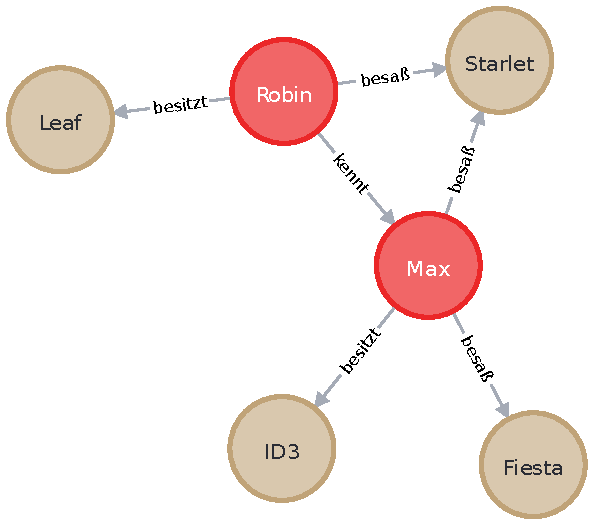
\includegraphics[width=0.75\textwidth]{images/example_graph.pdf}
    \caption{Beispiel Graph}
    \vspace{1em}
    \textit{Hier wird ein Beispiel Graph abgebildet der die Besitzbeziehungen zwischen einer Person (Besitzer) und einem Auto modelliert.}
    \label{fig:beispiel_graph}
\end{figure}

\subsection{Beziehungen}
\label{datenmodelle:beziehungen}
In diesem Abschnitt wird darauf eingegangen, wie und in welcher Form die Modelle Beziehungen zwischen Entitäten abbilden. 

\subsubsection{Relationales Modell}
Das relationale Modell unterstützt Beziehungen insofern, dass es möglich ist Beziehungen zwischen Entitätstypen zu definieren. Diese Beziehungen lassen sich dabei in die drei folgenden Kategorien unterteilen: 
\begin{itemize}
    \item \textit{one-to-one}, 
    \item \textit{one-to-many} (beziehungsweise \textit{many-to-one}) und 
    \item \textit{many-to-many}.
\end{itemize}

Bei der Repräsentation aller Beziehungskategorien spielen  folgenden Begriffe eine Schlüsselrolle:
\begin{itemize}
    \item \textit{Primärschlüssel}\\
    Beschreibt das Einzigartigkeitskriterium der Zeilen in einer Tabelle. Kann sich dabei auch aus mehreren Spalten zusammensetzen. 
    \item \textit{Sekundärschlüssel}\\
    Referenziert Zeilen einer anderen Tabelle B anhand des dortigen Primärschlüssels. Er gibt dabei an, welche Spalten von Tabelle A zur Referenz des Primärschlüssels genutzt werden. 
    \item \textit{Joins}\\
    Ermöglichen es solche Referenzen im Kontext einer Abfrage aufzulösen.
\end{itemize}

Bei \textit{one-to-one}- oder \textit{many-to-one}-Beziehungen genügt es, den oder die anderen Zeilen aus einer Tabelle mittels Sekundärschlüssel und Primärschlüssels zu referenzieren. Sollten die Informationen dann abgefragt werden, kann die Referenzierung durch einen Join aufgelöst werden.

Das Abbilden von \textit{many-to-many}-Beziehungen erfordert hingegen die Einführung einer Auflösungstabelle, siehe die Kfz-Register Tabelle in \autoref{fig:relationales_modell_many-to-many}. 

\begin{figure}[ht]
    \centering
    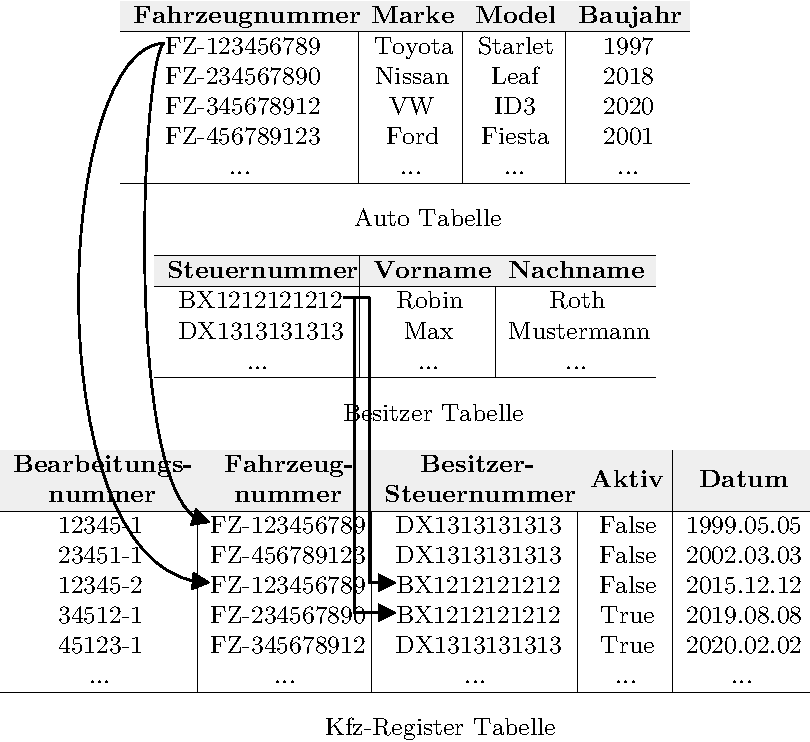
\includegraphics[width=\textwidth]{images/many-to-many.pdf}
    \caption{Beispiel many-to-many-Beziehungen im relationalen Modell}
    \label{fig:relationales_modell_many-to-many}
\end{figure}

\subsubsection{Graphmodell}
Beim Graphmodell stellen Beziehungen eine grundlegende Struktur in einem Graphen dar \cite{gdbms}, siehe \autoref{datenmodelle:structure}. Dabei werden im Graphmodell Beziehungen direkt zwischen Entitäten aufgebaut \cite{gdbms}, wie in \autoref{fig:beispiel_graph} erkennbar. 

Es unterstützt dadurch alle drei Beziehungskategorien, die aus dem relationalen Modell bekannt sind \textit{one-to-one}, \textit{many-to-one} und \textit{many-to-many}. Dabei findet im Graphmodell jedoch keinerlei Unterscheidung zwischen den drei Kategorien statt. Denn zwei Knoten können mehrere Edges haben, die sie miteinander verbinden. Dies ändert aber nichts an Art der Abbildung oder Referenzierung von Informationen. Alle Beziehungen werden also immer in Form einer Kante zwischen einem Start- und Zielknoten repräsentiert \cite{gdbms}. Zugleich muss darauf hingewiesen werden, dass es sich bei einem Start- und einer Kante, um denselben Knoten handeln kann. 

\subsection{Abfragesprachen}
Im Rahmen dieses Unterabschnitts wird auf Abfragesprachen eingegangen. Dabei werden die Abfragesprachen aufgeführt, die in Datenbanksystemen mit dem jeweiligen Datenmodell verbreitet sind.

\subsubsection{Relationales Modell}
Im Feld der relationalen Datenbanksysteme ist die Abfragesprache SQL weit verbreitet \cite{sql_history}. Sie wurde von Donald D. Chamberlin und Raymond F. Boyce im Rahmen des \textit{System R} Projekts entwickelt \cite{sql_history}. SQL wurde dabei mit der Motivation entworfen eine einfache Abfragesprache für relationale Daten zu entwickeln \cite{sql_history}. 

Bei SQL handelt es sich um eine deklarative Abfragesprache \cite{sql_history}. Der grundlegende Aufbau der Sprache und die Syntax können dabei \autoref{src:sql_example} entnommen werden. So ist in \autoref{src:sql_example} klar erkennbar, dass sich alle Operationen auf Tabellen und Spalten beziehen. Dabei arbeitet die Sprache -- wie erwartet -- in den Strukturen des relationalen Modells.

\begin{lstlisting}[caption={Beispiel SQL-Queries},language=SQL,label=src:sql_example]
/* Tabelle erstellen */
CREATE TABLE Autos (
    Fahrzeugnummer VARCHAR(50), 
    Marke VARCHAR(10), 
    Modell VARCHAR(10), 
    Baujahr INT,
    PRIMARY KEY(Fahrzeugnummer)
);

/* Daten in Tabelle schreiben */
INSERT INTO Autos 
(Fahrzeugnummer, Marke, Modell, Baujahr) 
("FZ-123456789", "Toyota", "Starlet", 1997);

/* Daten Abfragen */
SELECT Marke, Model, Baujahr FROM Autos 
WHERE Fahrzeugnummer = "FZ-123456789";

/* Daten Loeschen */
DELETE FROM Autos WHERE Fahrzeugnummer = "FZ-123456789";
\end{lstlisting}

Des Weiteren muss darauf hingewiesen werden, dass SQL als Sprache standardisiert wurde \cite{sql_history}. Allerdings gibt es heute trotz des Standards weiterhin sogenannte SQL-Dialekte \cite{sql_2017}. So können sich einige SQL Sprachelemente je nach Datenbanksystem oder Hersteller weiterhin unterscheiden \cite{sql_2017}. 

\subsubsection{Graphmodell}

Im Umfeld der Graph-Datenbanken gibt es keine dominierende Abfragesprache, wie SQL bei den relationalen Datenbanksystemen. Dort haben verschiedene Datenbanksysteme häufig auch unterschiedliche Abfragesprachen. Bei Gremlin und Cypher handelt es sich hierbei um zwei Vertreter solcher Sprachen, die auch im weiteren Verlauf dieser Arbeit eine Rolle spielen. 

Bei Gremlin handelt es sich um eine Abfragesprache, die mit dem TinkerPop Projekt in Verbindung steht \cite{tinkerpop_2020}. Sie wird dabei von einigen Graphdatenbanksystemen genutzt. Dazu gehören sowohl Db2 Graph als auch Neo4j, die beide im Rahmen der Arbeit eine wichtige Rolle einnehmen. Für die Interaktion mit dem Graphen bietet Gremlin dabei zwei verschiedene Abfragestile \cite{gremlin_paper}. So ist es einerseits möglich imperativ einen sogenannten Graph-Traversal durchzuführen, um mit dem Graph zu interagieren \cite{gremlin_paper}. Anderseits ist es allerdings auch möglich einen deklarativen Pattern-Matching-Stil zu wählen \cite{gremlin_paper}. Im Rahmen dieser Arbeit wurde bei Gremlin-Queries immer der imperative Graph-Traversal basierte Ansatz gewählt \cite{gremlin_paper}. Daher werden als Beispiel in \autoref{src:gremlin_example} lediglich imperative Queries aufgeführt. 

\begin{lstlisting}[caption={Beispiel Gremlin-Queries},language=JAVA,label=src:gremlin_example]
/* Daten in den Graph einfuegen */
v1 = g.addV('Auto').property('Modell','Leaf');
v2 = g.addV('Person').property('Name','Robin');
g.V(v1).addE('besitzt').to(v2).property('seit', '2019.08.08');

/* Daten abfragen */
g.V().hasLabel('Person').has('Name','Robin').outE('besitzt').outV().values('Modell')

/* Daten loeschen */
g.V().hasLabel("Person").has('Name', 'Max').drop();
\end{lstlisting}

Die Abfragesprache Cypher, wurde mit dem Ziel entworfen eine einfache, deklarative Art der Interaktion mit Graph-Daten zu ermöglichen \cite{gdbms}. Eine wichtige Sprachkomponente stellt dabei der Pattern-Matching-Stiel dar \cite{gdbms}. Von den beiden Datenbanksystemen Neo4j und Db2 Graph unterstützt allerdings nur Neo4j die Sprache -- zumindest direkt. In \autoref{src:cypher_example} werden hierbei einige Beispiel-Cypher-Queries aufgeführt. Diese sind mit den Gremlin-Queries in \autoref{src:gremlin_example} bezüglich ihrer Funktion vergleichbar. 

\begin{lstlisting}[caption={Beispiel Cypher-Queries},language=SQL,label=src:cypher_example]
/* Daten in den Graph einfuegen */
CREATE (:Person{name: "Robin"})-[:besitzt{seit: "2019.08.08"}]->(:Auto{modell: "Leaf"});

/* Daten abfragen */
MATCH (:Person{name: "Robin"})-[:besitzt]->(n2) RETURN n2.modell;

/* Daten loeschen */
MATCH (n:Person{name: "Robin"}) DETACH DELETE n;
\end{lstlisting}

\subsection{Zusammenfassung}

Beim relationalen und Graph-basierten Datenmodell handelt es sich um, zwei grundlegend verschiedene Modelle zur Abstraktion von Daten.

Datenbanksysteme, die auf dem relationalen Modell basieren, gibt es bereits deutlich länger als moderne Graph\-daten\-bank\-systeme. Darüber hinaus machen die relationale Vertreter auch den Großteil des Datenbankmarktes aus. Graphdatenbanksysteme hingegen weisen im Vergleich zu relationalen Systemen aktuell einen verschwindend geringen Marktanteil auf, stoßen jedoch auf immer größeres Interesse. 

Das relationale Modell fordert ein striktes Schema ein. Daten dürfen darin aufgrund des Informationsprinzips ausschließlich in einer bestimmten Weise repräsentiert werden. So hält das Modell die Daten in nach Entitätstyp getrennten Tabellen. Die Daten werden dabei in Tabellen auf Basis von Zeilen und Spalten organisiert. Das Graphmodell hingegen unterstützt ein flexibles Schema. Heterogene Daten können hierbei durch Vertexes und Edges in Graph abgebildet werden. 

Beim Graphmodell steht die Repräsentation von Beziehungen zwischen Daten bereits im Zentrum des Modells. So ist es möglich mittels einer Kante, die Beziehung zwischen zwei Entitäten (Knoten) zu modellieren. Beim relationalen Modell werden hingegen Entitätstypen miteinander in Beziehung gesetzt. Dies geschieht durch die Referenzierung einer Zeile einer anderen Tabelle anhand eines einzigartigen Merkmals.

Als Abfragesprache dominiert bei den relationalen Datenbanksystemen das deklarative SQL. Im Umfeld der Graphdatenbanksysteme existiert eine Vielzahl an Sprachen. Dazu gehören die für die Arbeit relevanten Abfragesprachen Gremlin und Cypher. 